\begin{frame}[fragile]{Verification Approaches}
    \centering
    \begin{figure}
        \begin{subfigure}{0.33\textwidth}
            \centering
            \resizebox{0.5\textwidth}{!}{
            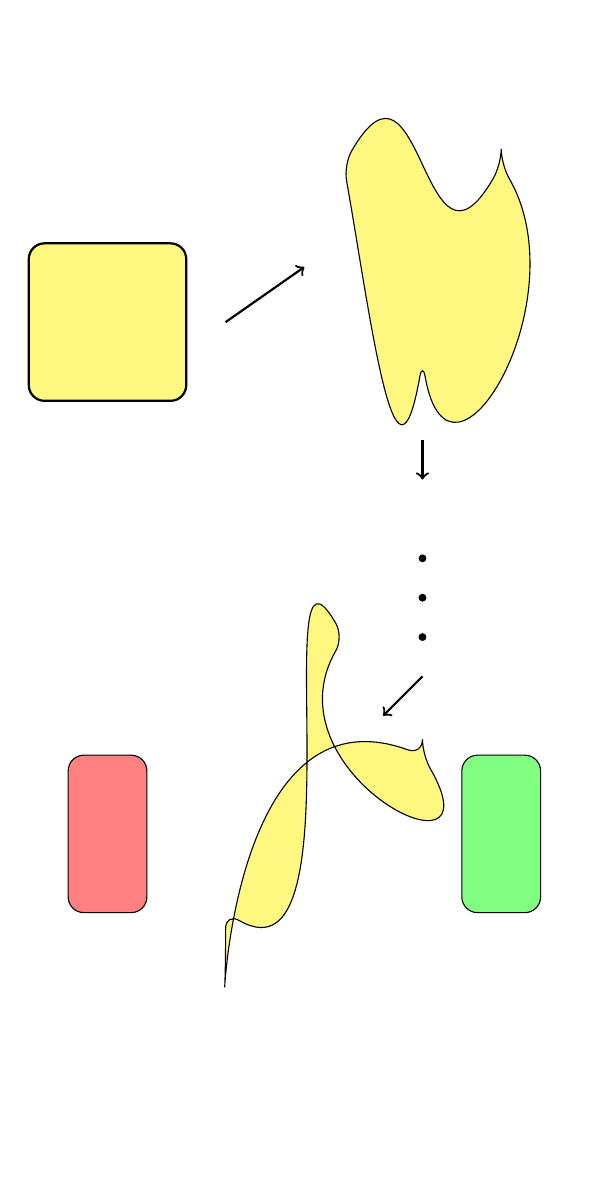
\begin{tikzpicture}
                \def\b{1};
                \draw[fill=yellow!50, rounded corners=2mm] 
                (\b,2.5) .. controls +(-60:2) and +(-80:2) .. 
                (0,0) .. controls +(-100:2) and +(-80:2) .. 
                (-\b,2.5) .. controls +(60:2) and +(-120:2) ..
                cycle;    
                % Draw the rectangle to the left of the Bézier curve
                \draw[thick, rounded corners=2mm, fill=yellow!50] 
                (-\b-4,-0.5) rectangle (-\b-2,1.5);
                % Draw three dots symbolizing the \ldots command
                \foreach \y in {-2.5, -3, -3.5} {
                \fill (0, \y) circle (0.05);
                }
                \draw[fill=yellow!50, rounded corners=2mm] 
                (0,-5) .. controls +(-20:-3) and +(90:-3) .. 
                (-2.5,-7) .. controls +(150:-2) and +(-60:-2) .. 
                (-\b,-3.5) .. controls +(60:-2) and +(120:-2) ..
                cycle;    

                % Draw an arrow between the rectangle and the Bézier shape
                \draw[thick, ->] (-\b-1.5, 0.5) -- (-\b-0.5, 1.2);
                \draw[thick, ->] (0, -1) -- (0, -1.5);
                \draw[thick, ->] (0, -4) -- (-0.5, -4.5);

                %Draw a goal set 
                \draw[fill=green!50, rounded corners=2mm] 
                (0.5,-5) rectangle (1.5,-7);

                %Draw an avoid set
                \draw[fill=red!50, rounded corners=2mm] 
                (-3.5,-5) rectangle (-4.5,-7);

            \end{tikzpicture}
            }
            \caption{Reachability Analysis}
        \end{subfigure}
        \begin{subfigure}{0.33\textwidth}
            \centering
            \resizebox{\textwidth}{!}{
            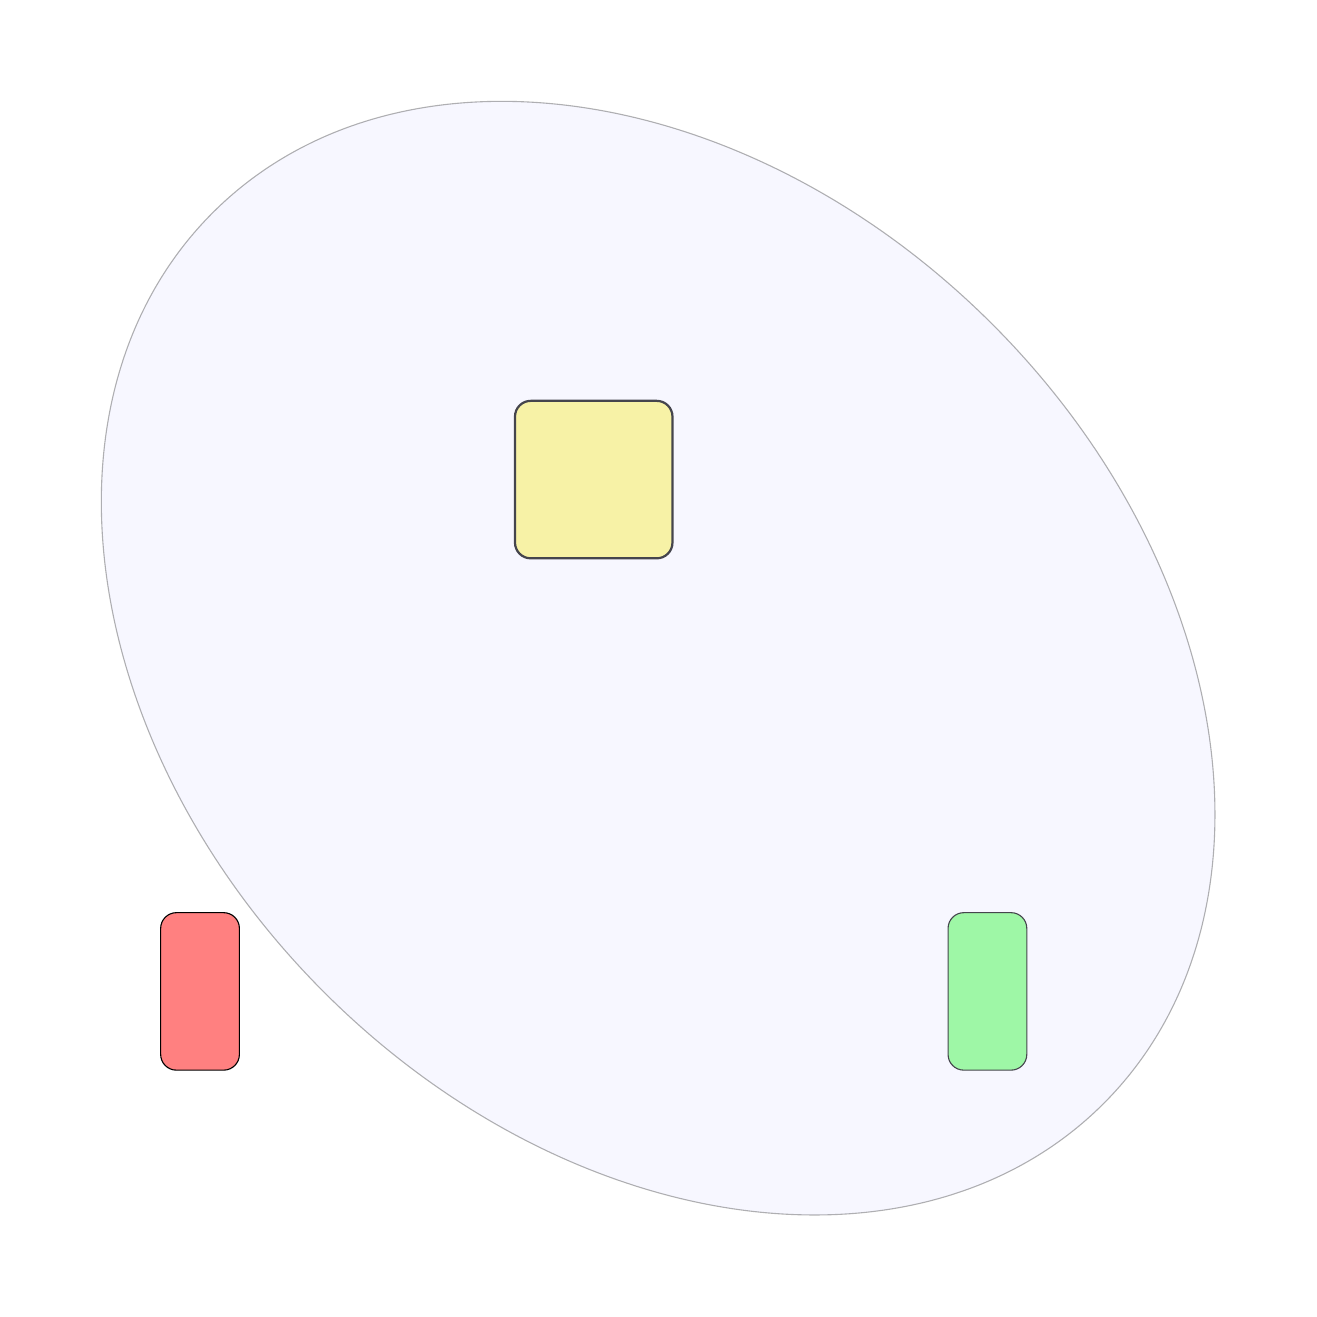
\begin{tikzpicture}
                \def\b{1};
                % Draw the rectangle to the left of the Bézier curve
                \draw[thick, rounded corners=2mm, fill=yellow!50] 
                (-\b-4,-0.5) rectangle (-\b-2,1.5);

                %Draw a goal set 
                \draw[fill=green!50, rounded corners=2mm] 
                (0.5,-5) rectangle (1.5,-7);

                %Draw an avoid set
                \draw[fill=red!50, rounded corners=2mm] 
                (-9.5,-5) rectangle (-8.5,-7);

                %Draw an invariant ellipse 
                \draw[fill=blue!10, opacity=0.3, rounded corners=2mm, rotate=-45] 
                (-1,-3.5) ellipse (8 and 6);

            \end{tikzpicture}
            }
            \caption{Invariance Analysis}
        \end{subfigure}
        \begin{subfigure}{0.3\textwidth}
            \centering
            \resizebox{\textwidth}{!}{
            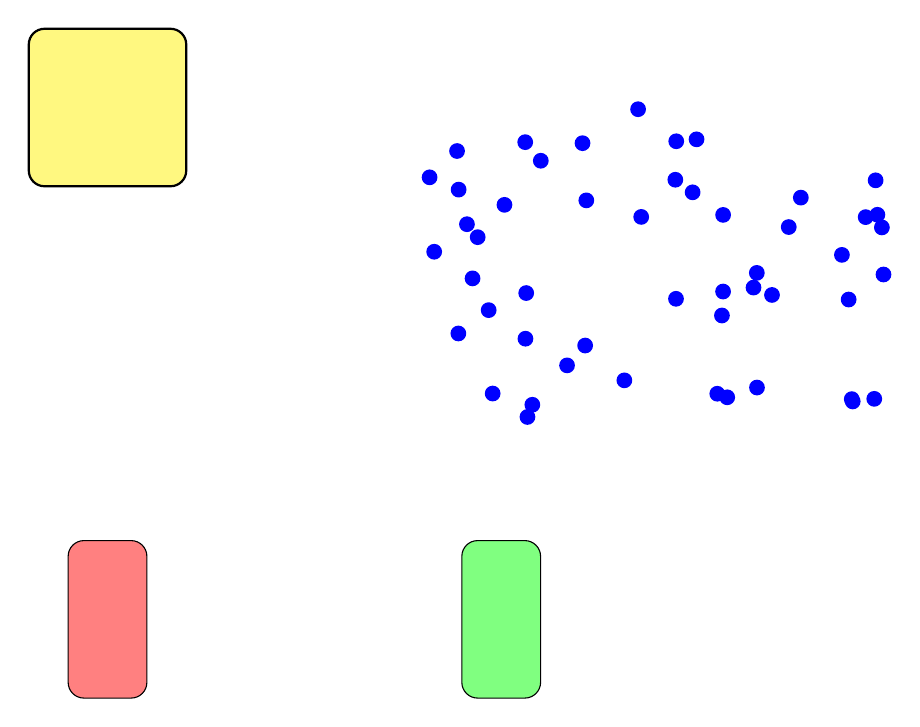
\begin{tikzpicture}
                \def\b{1};
                % Draw the rectangle to the left of the Bézier curve
                \draw[thick, rounded corners=2mm, fill=yellow!50] 
                (-\b-4,-0.5) rectangle (-\b-2,1.5);

                %Draw a goal set 
                \draw[fill=green!50, rounded corners=2mm] 
                (0.5,-5) rectangle (1.5,-7);

                %Draw an avoid set
                \draw[fill=red!50, rounded corners=2mm] 
                (-3.5,-5) rectangle (-4.5,-7);

                    % Plot random samples inside the ellipse
                \foreach \i in {1,...,50} {
                    \pgfmathsetmacro\xr{rnd*6} % Random x within ellipse's width
                    \pgfmathsetmacro\yr{rnd*4} % Random y within ellipse's height
                    \fill[blue] (0+\xr, -3.5+\yr) circle (0.1);
                }
            \end{tikzpicture}
            }
            \caption{Falsification}
        \end{subfigure}
    \end{figure}
\end{frame}

\begin{frame}[fragile]{Reachability Approaches}
    \begin{figure}
        \begin{subfigure}{0.4\textwidth}
            \centering
            \resizebox{0.4\textwidth}{!}{
            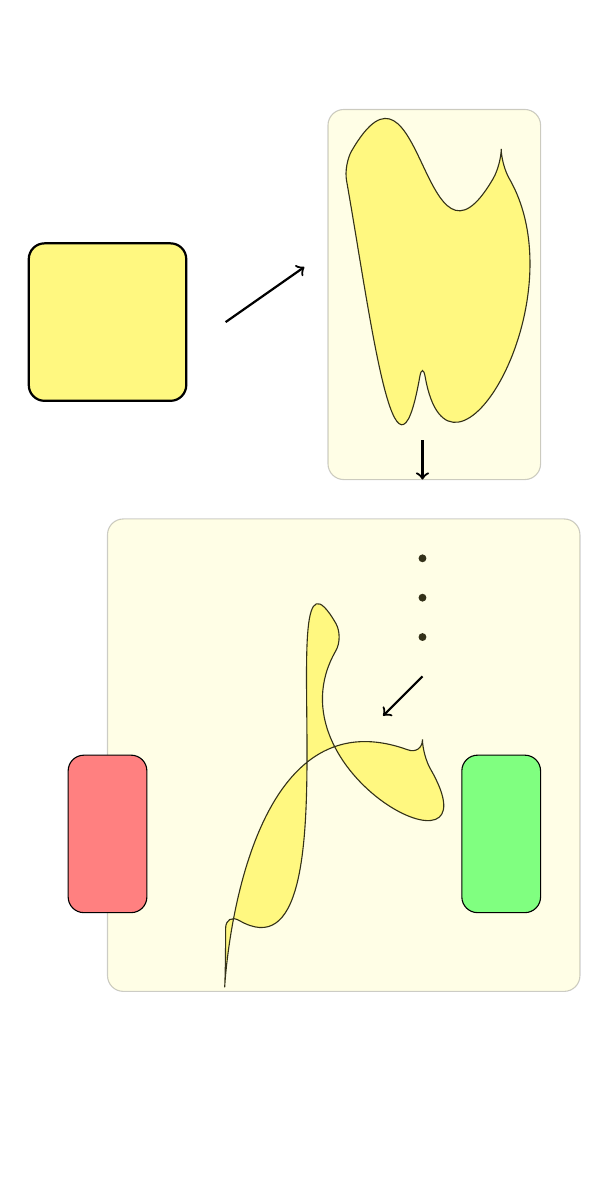
\begin{tikzpicture}
                \def\b{1};
                \draw[fill=yellow!50, rounded corners=2mm] 
                (\b,2.5) .. controls +(-60:2) and +(-80:2) .. 
                (0,0) .. controls +(-100:2) and +(-80:2) .. 
                (-\b,2.5) .. controls +(60:2) and +(-120:2) ..
                cycle;    

                \draw[fill=yellow!50, rounded corners=2mm, opacity=0.2] 
                (-\b-0.2, -1.5) rectangle (\b+0.5, 3.2);
                % Draw the rectangle to the left of the Bézier curve
                \draw[thick, rounded corners=2mm, fill=yellow!50] 
                (-\b-4,-0.5) rectangle (-\b-2,1.5);
                % Draw three dots symbolizing the \ldots command
                \foreach \y in {-2.5, -3, -3.5} {
                \fill (0, \y) circle (0.05);
                }
                \draw[fill=yellow!50, rounded corners=2mm] 
                (0,-5) .. controls +(-20:-3) and +(90:-3) .. 
                (-2.5,-7) .. controls +(150:-2) and +(-60:-2) .. 
                (-\b,-3.5) .. controls +(60:-2) and +(120:-2) ..
                cycle; 
                \draw[fill=yellow!50, rounded corners=2mm, opacity=0.2] 
                (-4, -8) rectangle (2, -2);   

                % Draw an arrow between the rectangle and the Bézier shape
                \draw[thick, ->] (-\b-1.5, 0.5) -- (-\b-0.5, 1.2);
                \draw[thick, ->] (0, -1) -- (0, -1.5);
                \draw[thick, ->] (0, -4) -- (-0.5, -4.5);

                %Draw a goal set 
                \draw[fill=green!50, rounded corners=2mm] 
                (0.5,-5) rectangle (1.5,-7);

                %Draw an avoid set
                \draw[fill=red!50, rounded corners=2mm] 
                (-3.5,-5) rectangle (-4.5,-7);

            \end{tikzpicture}
            }
            \caption{Abstraction Propagation}
        \end{subfigure}
        \begin{subfigure}{0.4\textwidth}
            \centering
            \resizebox{0.4\textwidth}{!}{
                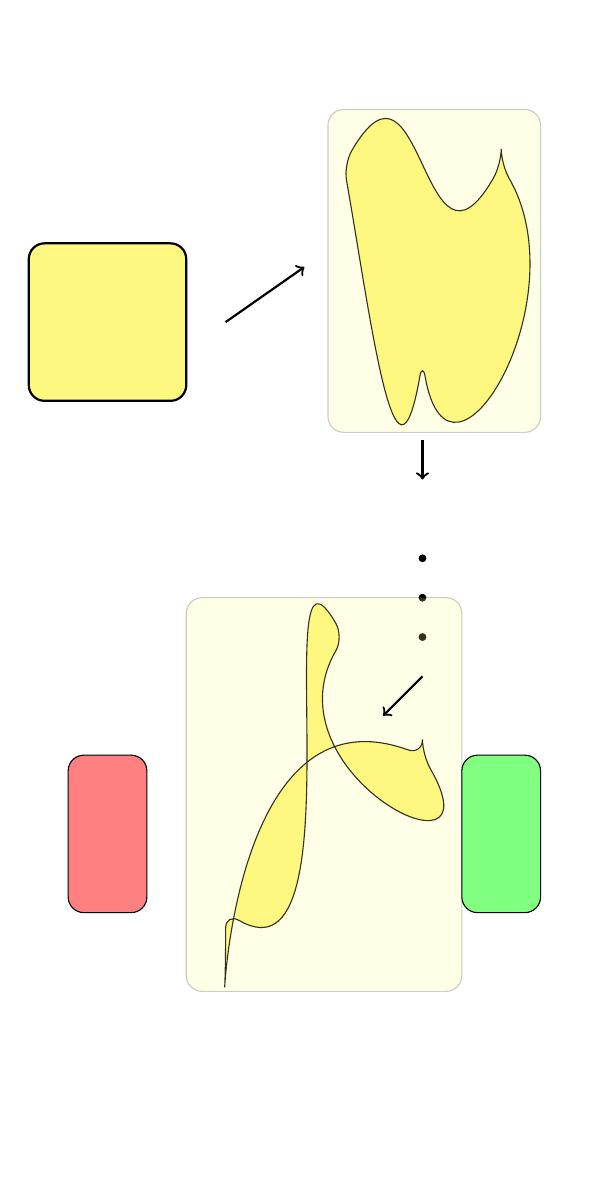
\begin{tikzpicture}
                    \def\b{1};
                    \draw[fill=yellow!50, rounded corners=2mm] 
                    (\b,2.5) .. controls +(-60:2) and +(-80:2) .. 
                    (0,0) .. controls +(-100:2) and +(-80:2) .. 
                    (-\b,2.5) .. controls +(60:2) and +(-120:2) ..
                    cycle;    
    
                    \draw[fill=yellow!50, rounded corners=2mm, opacity=0.2] 
                    (-\b-0.2, -0.9) rectangle (\b+0.5, 3.2);
                    % Draw the rectangle to the left of the Bézier curve
                    \draw[thick, rounded corners=2mm, fill=yellow!50] 
                    (-\b-4,-0.5) rectangle (-\b-2,1.5);
                    % Draw three dots symbolizing the \ldots command
                    \foreach \y in {-2.5, -3, -3.5} {
                    \fill (0, \y) circle (0.05);
                    }
                    \draw[fill=yellow!50, rounded corners=2mm] 
                    (0,-5) .. controls +(-20:-3) and +(90:-3) .. 
                    (-2.5,-7) .. controls +(150:-2) and +(-60:-2) .. 
                    (-\b,-3.5) .. controls +(60:-2) and +(120:-2) ..
                    cycle; 
                    \draw[fill=yellow!50, rounded corners=2mm, opacity=0.2] 
                    (-3, -8) rectangle (0.5, -3);   
    
                    % Draw an arrow between the rectangle and the Bézier shape
                    \draw[thick, ->] (-\b-1.5, 0.5) -- (-\b-0.5, 1.2);
                    \draw[thick, ->] (0, -1) -- (0, -1.5);
                    \draw[thick, ->] (0, -4) -- (-0.5, -4.5);
    
                    %Draw a goal set 
                    \draw[fill=green!50, rounded corners=2mm] 
                    (0.5,-5) rectangle (1.5,-7);
    
                    %Draw an avoid set
                    \draw[fill=red!50, rounded corners=2mm] 
                    (-3.5,-5) rectangle (-4.5,-7);
    
                \end{tikzpicture}
            }
            \caption{Combinatorial Optimization}
        \end{subfigure}
    \end{figure}
\end{frame}

\begin{frame}[fragile]{Abstraction Propagation}
    \begin{columns}
        \begin{column}{0.4\textwidth}
            \begin{figure}
                \centering
                \resizebox{0.4\textwidth}{!}{
                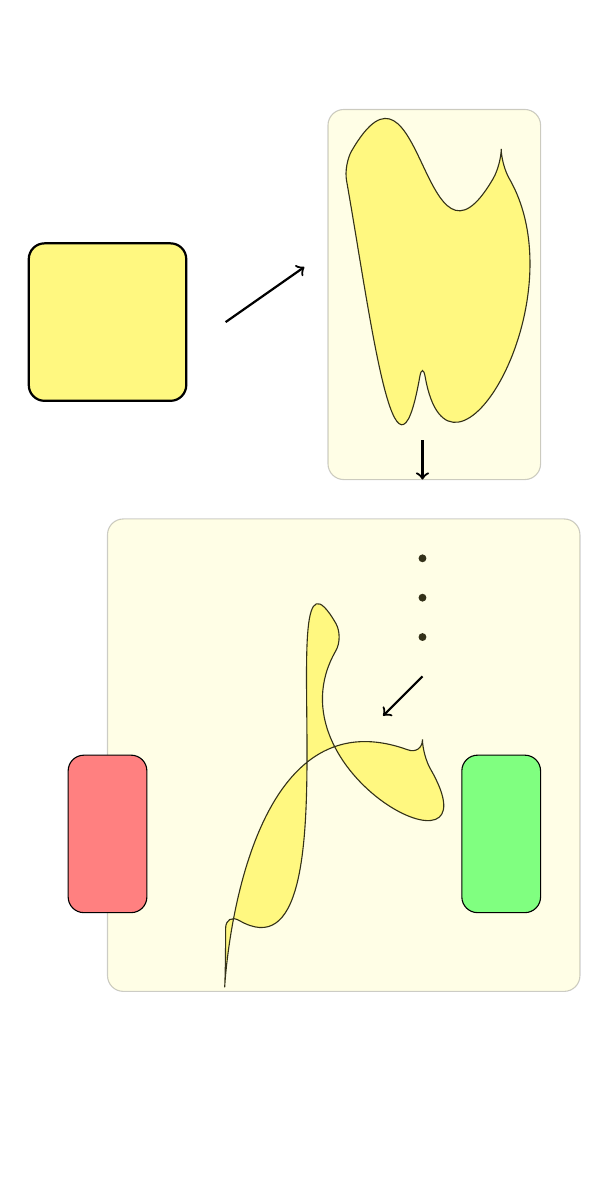
\begin{tikzpicture}
                    \def\b{1};
                    \draw[fill=yellow!50, rounded corners=2mm] 
                    (\b,2.5) .. controls +(-60:2) and +(-80:2) .. 
                    (0,0) .. controls +(-100:2) and +(-80:2) .. 
                    (-\b,2.5) .. controls +(60:2) and +(-120:2) ..
                    cycle;    
    
                    \draw[fill=yellow!50, rounded corners=2mm, opacity=0.2] 
                    (-\b-0.2, -1.5) rectangle (\b+0.5, 3.2);
                    % Draw the rectangle to the left of the Bézier curve
                    \draw[thick, rounded corners=2mm, fill=yellow!50] 
                    (-\b-4,-0.5) rectangle (-\b-2,1.5);
                    % Draw three dots symbolizing the \ldots command
                    \foreach \y in {-2.5, -3, -3.5} {
                    \fill (0, \y) circle (0.05);
                    }
                    \draw[fill=yellow!50, rounded corners=2mm] 
                    (0,-5) .. controls +(-20:-3) and +(90:-3) .. 
                    (-2.5,-7) .. controls +(150:-2) and +(-60:-2) .. 
                    (-\b,-3.5) .. controls +(60:-2) and +(120:-2) ..
                    cycle; 
                    \draw[fill=yellow!50, rounded corners=2mm, opacity=0.2] 
                    (-4, -8) rectangle (2, -2);   
    
                    % Draw an arrow between the rectangle and the Bézier shape
                    \draw[thick, ->] (-\b-1.5, 0.5) -- (-\b-0.5, 1.2);
                    \draw[thick, ->] (0, -1) -- (0, -1.5);
                    \draw[thick, ->] (0, -4) -- (-0.5, -4.5);
    
                    %Draw a goal set 
                    \draw[fill=green!50, rounded corners=2mm] 
                    (0.5,-5) rectangle (1.5,-7);
    
                    %Draw an avoid set
                    \draw[fill=red!50, rounded corners=2mm] 
                    (-3.5,-5) rectangle (-4.5,-7);
    
                \end{tikzpicture}
                }
            \end{figure}
        \end{column}
        \begin{column}{0.6\textwidth}
            Tools using these methods propagate an abstract representation of the system to compute reachable sets.
            
            \vspace{0.5cm}

            Representations include: Taylor models, Bernstein polynomials, zonotopes, and polytopes.

            \vspace{0.5cm}

            The CORA tool\footcite{kochdumper2023constrained} is a representative example of this approach.
        \end{column}
    \end{columns}
\end{frame}

\begin{frame}[fragile]{Limitations: Abstraction Propagation}
    \begin{columns}
        \begin{column}{0.4\textwidth}
            \begin{figure}
                \centering
                \resizebox{0.4\textwidth}{!}{
                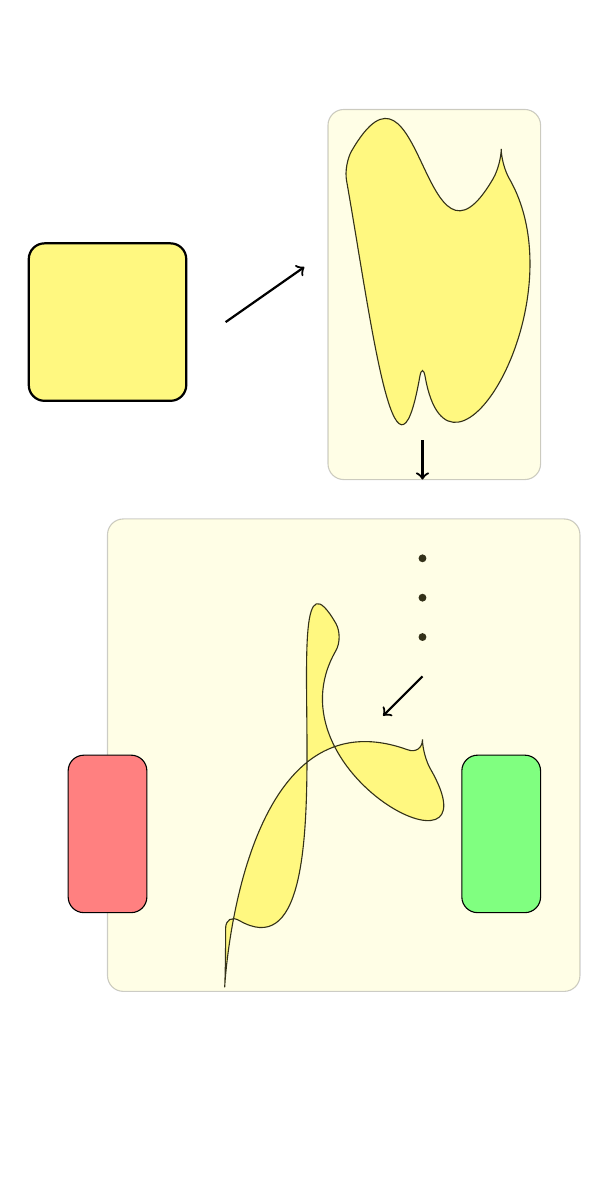
\begin{tikzpicture}
                    \def\b{1};
                    \draw[fill=yellow!50, rounded corners=2mm] 
                    (\b,2.5) .. controls +(-60:2) and +(-80:2) .. 
                    (0,0) .. controls +(-100:2) and +(-80:2) .. 
                    (-\b,2.5) .. controls +(60:2) and +(-120:2) ..
                    cycle;    
    
                    \draw[fill=yellow!50, rounded corners=2mm, opacity=0.2] 
                    (-\b-0.2, -1.5) rectangle (\b+0.5, 3.2);
                    % Draw the rectangle to the left of the Bézier curve
                    \draw[thick, rounded corners=2mm, fill=yellow!50] 
                    (-\b-4,-0.5) rectangle (-\b-2,1.5);
                    % Draw three dots symbolizing the \ldots command
                    \foreach \y in {-2.5, -3, -3.5} {
                    \fill (0, \y) circle (0.05);
                    }
                    \draw[fill=yellow!50, rounded corners=2mm] 
                    (0,-5) .. controls +(-20:-3) and +(90:-3) .. 
                    (-2.5,-7) .. controls +(150:-2) and +(-60:-2) .. 
                    (-\b,-3.5) .. controls +(60:-2) and +(120:-2) ..
                    cycle; 
                    \draw[fill=yellow!50, rounded corners=2mm, opacity=0.2] 
                    (-4, -8) rectangle (2, -2);   
    
                    % Draw an arrow between the rectangle and the Bézier shape
                    \draw[thick, ->] (-\b-1.5, 0.5) -- (-\b-0.5, 1.2);
                    \draw[thick, ->] (0, -1) -- (0, -1.5);
                    \draw[thick, ->] (0, -4) -- (-0.5, -4.5);
    
                    %Draw a goal set 
                    \draw[fill=green!50, rounded corners=2mm] 
                    (0.5,-5) rectangle (1.5,-7);
    
                    %Draw an avoid set
                    \draw[fill=red!50, rounded corners=2mm] 
                    (-3.5,-5) rectangle (-4.5,-7);
    
                \end{tikzpicture}
                }
            \end{figure}
        \end{column}
        \begin{column}{0.6\textwidth}
            Abstraction propagation can be computationally efficient, but the inexactness of the abstraction often leads to excess conservatism
            
            \vspace{0.5cm}

            This especially affects systems with nonlinear dynamics, and long time horizons.
        \end{column}
    \end{columns}
\end{frame}

\begin{frame}[fragile]{Combinatorial Optimization}
    \begin{columns}
        \begin{column}{0.4\textwidth}
            \begin{figure}
                \centering
                \resizebox{0.4\textwidth}{!}{
                    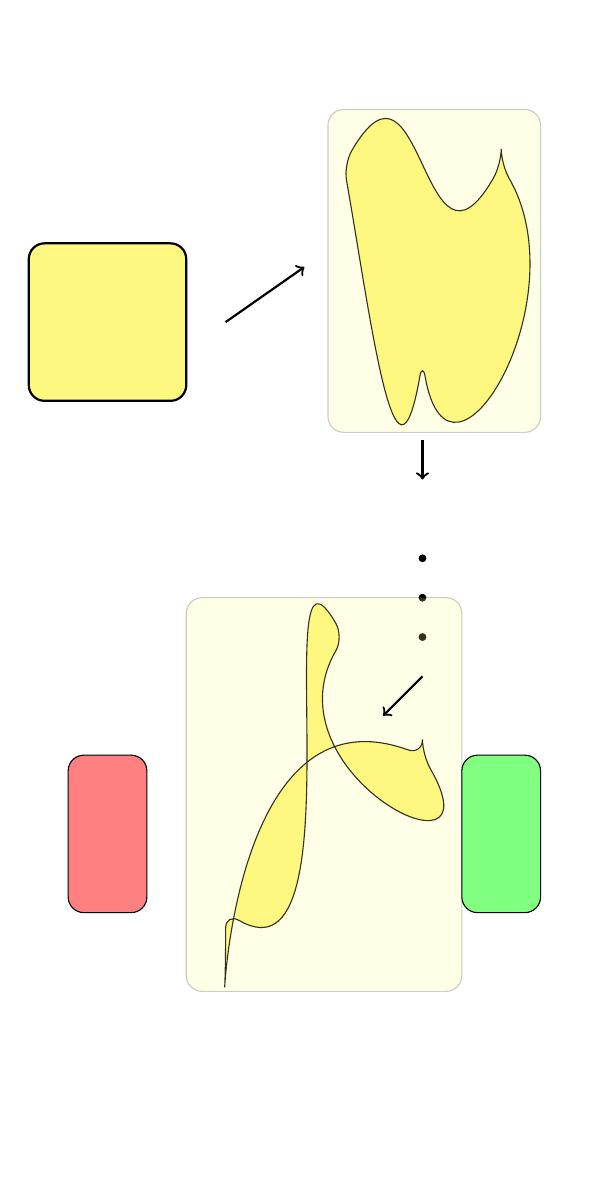
\begin{tikzpicture}
                        \def\b{1};
                        \draw[fill=yellow!50, rounded corners=2mm] 
                        (\b,2.5) .. controls +(-60:2) and +(-80:2) .. 
                        (0,0) .. controls +(-100:2) and +(-80:2) .. 
                        (-\b,2.5) .. controls +(60:2) and +(-120:2) ..
                        cycle;    
        
                        \draw[fill=yellow!50, rounded corners=2mm, opacity=0.2] 
                        (-\b-0.2, -0.9) rectangle (\b+0.5, 3.2);
                        % Draw the rectangle to the left of the Bézier curve
                        \draw[thick, rounded corners=2mm, fill=yellow!50] 
                        (-\b-4,-0.5) rectangle (-\b-2,1.5);
                        % Draw three dots symbolizing the \ldots command
                        \foreach \y in {-2.5, -3, -3.5} {
                        \fill (0, \y) circle (0.05);
                        }
                        \draw[fill=yellow!50, rounded corners=2mm] 
                        (0,-5) .. controls +(-20:-3) and +(90:-3) .. 
                        (-2.5,-7) .. controls +(150:-2) and +(-60:-2) .. 
                        (-\b,-3.5) .. controls +(60:-2) and +(120:-2) ..
                        cycle; 
                        \draw[fill=yellow!50, rounded corners=2mm, opacity=0.2] 
                        (-3, -8) rectangle (0.5, -3);   
        
                        % Draw an arrow between the rectangle and the Bézier shape
                        \draw[thick, ->] (-\b-1.5, 0.5) -- (-\b-0.5, 1.2);
                        \draw[thick, ->] (0, -1) -- (0, -1.5);
                        \draw[thick, ->] (0, -4) -- (-0.5, -4.5);
        
                        %Draw a goal set 
                        \draw[fill=green!50, rounded corners=2mm] 
                        (0.5,-5) rectangle (1.5,-7);
        
                        %Draw an avoid set
                        \draw[fill=red!50, rounded corners=2mm] 
                        (-3.5,-5) rectangle (-4.5,-7);
        
                    \end{tikzpicture}
                }
            \end{figure}
        \end{column}
        \begin{column}{0.6\textwidth}
            Tools using these methods solve combinatorial problems to compute reachable sets.
            
            \vspace{0.5cm}

            They often represent the system as integer programs, hybrid zonotopes, or marching trees.

            \vspace{0.5cm}

            The OVERTVerify tool \footcite{sidrane2022overt} is a representative example of this approach.
        \end{column}
    \end{columns}
\end{frame}

\begin{frame}[fragile]{Limitations: Combinatorial Optimization}
    \begin{columns}
        \begin{column}{0.4\textwidth}
            \begin{figure}
                \centering
                \resizebox{0.4\textwidth}{!}{
                    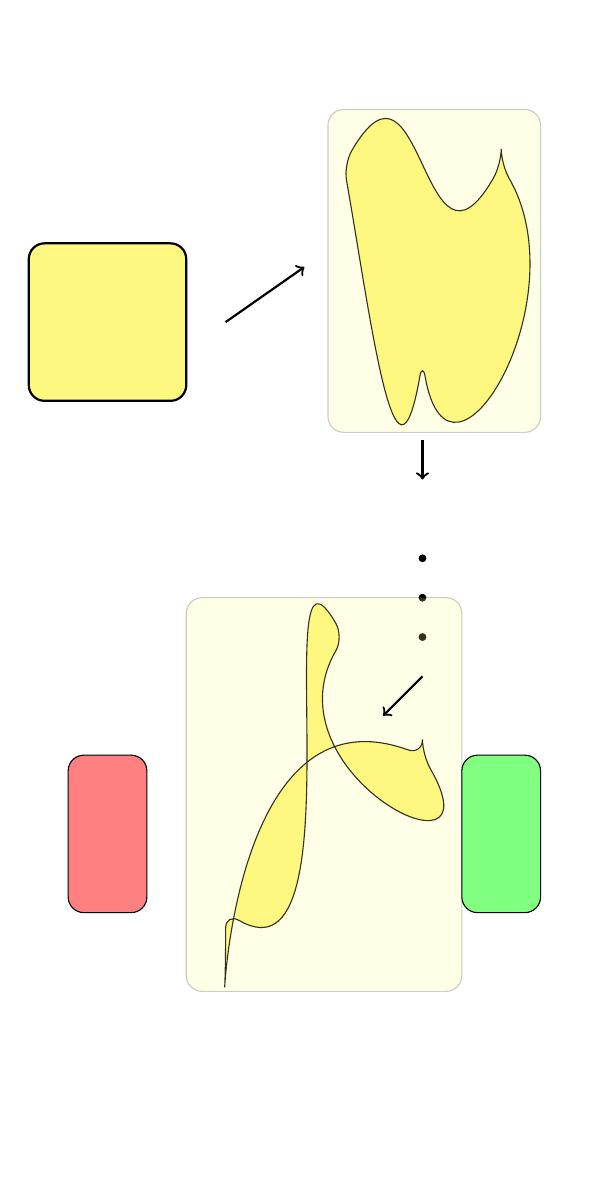
\begin{tikzpicture}
                        \def\b{1};
                        \draw[fill=yellow!50, rounded corners=2mm] 
                        (\b,2.5) .. controls +(-60:2) and +(-80:2) .. 
                        (0,0) .. controls +(-100:2) and +(-80:2) .. 
                        (-\b,2.5) .. controls +(60:2) and +(-120:2) ..
                        cycle;    
        
                        \draw[fill=yellow!50, rounded corners=2mm, opacity=0.2] 
                        (-\b-0.2, -0.9) rectangle (\b+0.5, 3.2);
                        % Draw the rectangle to the left of the Bézier curve
                        \draw[thick, rounded corners=2mm, fill=yellow!50] 
                        (-\b-4,-0.5) rectangle (-\b-2,1.5);
                        % Draw three dots symbolizing the \ldots command
                        \foreach \y in {-2.5, -3, -3.5} {
                        \fill (0, \y) circle (0.05);
                        }
                        \draw[fill=yellow!50, rounded corners=2mm] 
                        (0,-5) .. controls +(-20:-3) and +(90:-3) .. 
                        (-2.5,-7) .. controls +(150:-2) and +(-60:-2) .. 
                        (-\b,-3.5) .. controls +(60:-2) and +(120:-2) ..
                        cycle; 
                        \draw[fill=yellow!50, rounded corners=2mm, opacity=0.2] 
                        (-3, -8) rectangle (0.5, -3);   
        
                        % Draw an arrow between the rectangle and the Bézier shape
                        \draw[thick, ->] (-\b-1.5, 0.5) -- (-\b-0.5, 1.2);
                        \draw[thick, ->] (0, -1) -- (0, -1.5);
                        \draw[thick, ->] (0, -4) -- (-0.5, -4.5);
        
                        %Draw a goal set 
                        \draw[fill=green!50, rounded corners=2mm] 
                        (0.5,-5) rectangle (1.5,-7);
        
                        %Draw an avoid set
                        \draw[fill=red!50, rounded corners=2mm] 
                        (-3.5,-5) rectangle (-4.5,-7);
        
                    \end{tikzpicture}
                }
            \end{figure}
        \end{column}
        \begin{column}{0.6\textwidth}
            While combinatorial optimization can be arbitrarily precise, computing reachable sets is computationally expensive.
            
            \vspace{0.5cm}

            The problem quickly becomes intractable when the system dynamics are nonlinear, or the time horizon is long.
        \end{column}
    \end{columns}
\end{frame}